\documentclass{article}

\usepackage{fancyhdr} % Required for custom headers
\usepackage{lastpage} % Required to determine the last page for the footer
\usepackage{extramarks} % Required for headers and footers
\usepackage[usenames,dvipsnames]{color} % Required for custom colors
\usepackage{graphicx} % Required to insert images
\usepackage{listings} % Required for insertion of code
\usepackage{courier} % Required for the courier font
\usepackage{lipsum} % Used for inserting dummy 'Lorem ipsum' text into the template
\usepackage{hyperref}
% Margins
\topmargin=-0.45in
\evensidemargin=0in
\oddsidemargin=0in
\textwidth=6.5in
\textheight=9.0in
\headsep=0.25in

\linespread{1.1} % Line spacing

% Set up the header and footer
\pagestyle{fancy}
\lhead{\hmwkAuthorName} % Top left header
\chead{\hmwkClass\ (\hmwkClassInstructor\ \hmwkClassTime): \hmwkTitle} % Top center head
\rhead{\firstxmark} % Top right header
\lfoot{\lastxmark} % Bottom left footer
\cfoot{} % Bottom center footer
\rfoot{Page\ \thepage\ of\ \protect\pageref{LastPage}} % Bottom right footer
\renewcommand\headrulewidth{0.4pt} % Size of the header rule
\renewcommand\footrulewidth{0.4pt} % Size of the footer rule

\setlength\parindent{0pt} % Removes all indentation from paragraphs

\usepackage{listings}
\usepackage{color}

\definecolor{dkgreen}{rgb}{0,0.6,0}
\definecolor{gray}{rgb}{0.5,0.5,0.5}
\definecolor{mauve}{rgb}{0.58,0,0.82}

\lstset{frame=tb,
  language=Java,
  aboveskip=3mm,
  belowskip=3mm,
  showstringspaces=false,
  columns=flexible,
  basicstyle={\small\ttfamily},
  numbers=none,
  numberstyle=\tiny\color{gray},
  keywordstyle=\color{blue},
  commentstyle=\color{dkgreen},
  stringstyle=\color{mauve},
  breaklines=true,
  breakatwhitespace=true
  tabsize=3
}

%------------------------------------------------------------------------------------------
%	DOCUMENT STRUCTURE COMMANDS
%	Skip this unless you know what you're doing
%-------------------------------------------------------------------------------------------

% Header and footer for when a page split occurs within a problem environment
\newcommand{\enterProblemHeader}[1]{
\nobreak\extramarks{#1}{#1 continued on next page\ldots}\nobreak
\nobreak\extramarks{#1 (continued)}{#1 continued on next page\ldots}\nobreak
}

% Header and footer for when a page split occurs between problem environments
\newcommand{\exitProblemHeader}[1]{
\nobreak\extramarks{#1 (continued)}{#1 continued on next page\ldots}\nobreak
\nobreak\extramarks{#1}{}\nobreak
}



%-------------------------------------------------------------------------------------------
%	NAME AND CLASS SECTION
%-------------------------------------------------------------------------------------------

\newcommand{\hmwkTitle}{UML and Sonar} % Assignment title
\newcommand{\hmwkDueDate}{Martedi,\ Aprile 29,\ 2014} % Due date
\newcommand{\hmwkClass}{Ingegneria del Software 1} % Course/class
\newcommand{\hmwkClassTime}{} % Class/lecture time
\newcommand{\hmwkClassInstructor}{} % Teacher/lecturer
\newcommand{\hmwkAuthorName}{} % Your name

%-------------------------------------------------------------------------------------------
%	TITLE PAGE
%-------------------------------------------------------------------------------------------

\title{
\vspace{2in}
\textmd{\textbf{\hmwkClass:\ \hmwkTitle}}\\
\normalsize\vspace{0.1in}\small{Due\ on\ \hmwkDueDate}\\
\vspace{0.1in}\large{\textit{\hmwkClassInstructor\ \hmwkClassTime}}
\vspace{3in}
}

\author{\textbf{\hmwkAuthorName}}
\date{} % Insert date here if you want it to appear below your name

%-------------------------------------------------------------------------------------------

\begin{document}

\maketitle

%-------------------------------------------------------------------------------------------
%	TABLE OF CONTENTS
%-------------------------------------------------------------------------------------------

%\setcounter{tocdepth}{1} % Uncomment this line if you don't want subsections listed in the ToC

\newpage
\tableofcontents
\newpage



%-------------------------------------------------------------------------------------------
\section{Introduction}
L'Unified Modeling Language (UML) \`e un linguaggio di modellazione di uso generale e fornisce uno strumento standard per progettare i nostri sistemi. 

I diagrammi UML forniscono due diverse informazioni sui nostri modelli:

\begin{enumerate}
\item Informazioni Statiche (o strutturali): forniscono una descrizione \emph{statica} del sistema utilizzando classi, attributi, operazioni e relazioni. I class diagram sono i diagrammi statici comunemente utilizzati.
\item Informazioni Dinamiche  (o comportamentali): descrivono il comportamento dinamico dell'applicazione mostrando le relazioni di collaborazione tra i vari oggetti e come lo stato interno degli oggetti cambia nel tempo. I sequence diagrams, activity diagrams e gli state machine diagrams sono diagrammi UML dinamici.
\end{enumerate}


\subsection{Class diagram}
I class Diagram descrivono la struttura del sistema, per mezzo di classi, attributi, operazioni (o metodi) e relazioni tra gli oggetti.\\

\subsubsection{Classe}
\begin{itemize}
\item  Le \textit{classi} sono illustrate per mezzo di rettangoli divisi verticalmente. Nella varie partizioni sono indicati:,
\begin{itemize}
\item il \emph{nome} della classe
\item gli \emph{attributi} della classe: sono le informazioni memorizzate nell'oggetto
\item i \emph{metodi}: sono operazioni che un oggetto pu\`o effettuare
\end{itemize}
\item Gli attributi e i metodi sono chiamati \emph{membri} della classe 
\item Ogni attributo e ogni metodo \`e associato a una visibilit\`a ovvero
\begin{itemize}
\item  $+$ Public,
\item  $-$ Private,
\item $\#$ Protected
\item  \~{} (Friendly).
\end{itemize}
\item possiamo specificare due tipi di cope per i membri della classe: instance and static.
\end{itemize}


\subsubsection{Associazione}
Rappresenta le relazioni statiche tra le classi. 
\begin{itemize}
\item L'associazione binaria (con 2 capi) \`e normalmente rappresentata per mezzo di una linea.
\item una associazione \`e solitamente labellata con un nome
\item i capi di una associazione sono solitamente decorati con indicatori di appartenenza, molteplicit\`a etc
\end{itemize}

\subsubsection{Aggregazione}
L'aggregazione \`e un particolare tipo di associazione utilizzata per descrivere una relazione di tipo "has a". In altre parole l' aggregazione \`e un tipo particolare di associazione che rappresenta la relazione tra una parte e il suo contenitore. L'aggregazione \`e utilizzata quando una classe \`e un contenitore di altre oggetti. Tuttavia contenitore e contenute non sono in una relazione ``forte" ovvero se il contenitore \`e distrutto le altri oggetti (contenuti) continuano ad esistere. 

\subsubsection{Composizione}
\`E un particolare tipo di aggregazione che viene utilizzato quando \`e presente una ``forte" relazione tra contenitore e contenuto. Se il contenitore viene distrutto ogni istanza degli oggetti contenuti viene distrutta di conseguenza.

\subsubsection{Generalizzazione}
\`E una relazione di tipo ``\`e un". Indica che una delle due classi (la sottoclasse) \`e considerata come una specializzazione dell'altra (la super classe). Questo significa che ogni istanza della sottoclasse \`e anche un istanza della super classe e che tutti i metodi pubblici e protetti della super classe sono ereditati dalla sotto classe. 

\subsubsection{Realizzazione}
\`E una relazione tra due modelli di elementi. Di solito una classe e un interfaccia, dove un elemento del modello (la classe) implementa il comportamento che altro elemento (l'interfaccia) specifica. Diverse classi possono ereditare il comportamento da una singola interfaccia.

\subsubsection{Dipendenza}
Indica che una delle classi dipende da un'altra classe perch\`e la utilizza in un certo istante di tempo. Una classe dipende da un altra se la utilizza come parametro o variabile locale in un metodo. 
\vspace{0.5cm}
\begin{center}
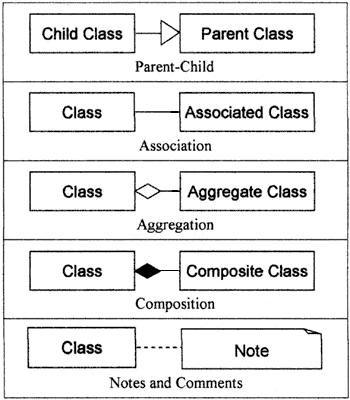
\includegraphics[scale=0.37]{class-not.png}\\
\end{center}
\subsection{Sequence diagram}

I sequence diagram descrivono l'interazione dinamica tra oggetti in un particolare scenario. Si rappresenta lo scambio di messaggi tra oggetti in sequenza temporale, dall'alto verso il basso. Ciascun oggetto coinvolto nello scenario presenta una \textit{lifeline} o linea di vita durante la quale pu\`o scambiare o ricevere messaggi da altri oggetti. La linea di vita  \`e rappresentata da una linea verticale tratteggiata che parte dall'oggetto. Un oggetto inizia una esecuzione (\textit{execution occurence}) quando viene coinvolto nelle interazioni dello scenario, ad esempio quando invia o riceve un messaggio. L'esecuzione si rappresenta sovrapponendo alla linea di vita un rettangolo solido esteso verticalmente fino al termine dell'esecuzione.


\begin{center}
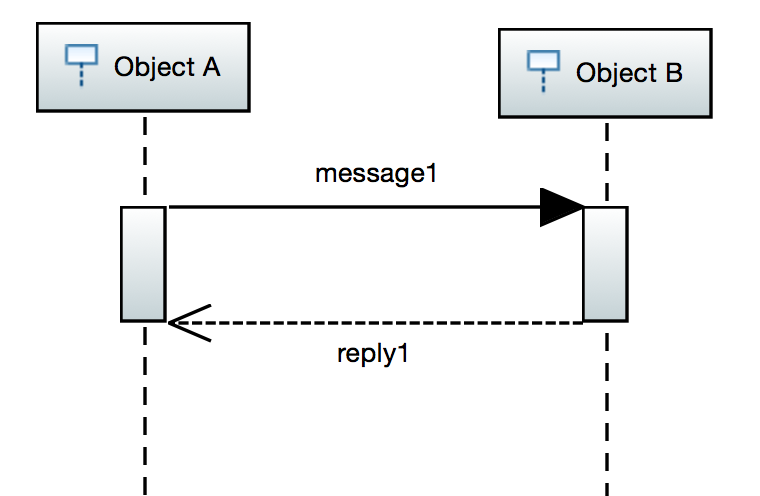
\includegraphics[scale=0.4]{seq-simple.png}\\
\end{center}


\subsubsection{Messaggi}

Lo scambio di messaggi si rappresenta con una freccia orizzontale dalla lifeline dell'oggetto chiamante a quella del ricevente. Lungo le frecce dei messaggi \`e possibile descrivere con un testo il tipo di messaggio (nome del metodo, argomenti, etc.). Esistono principalmente i seguenti tipi di messaggio:

\begin{itemize}
\item  \textit{Messaggio sincrono}: un messaggio, come la classica chiamata ad un metodo, che blocca il chiamante fino alla ricezione della risposta 
\item  \textit{Messaggio asincrono}: un messaggio non bloccante
\item  \textit{Messaggio di ritorno}: la risposta ad un messaggio sincrono o asincrono (callback)
\item  \textit{Messaggio di creazione}: messaggio che rappresenta la creazione di un oggetto
\item  \textit{Messaggio di distruzione}: messaggio che rappresenta la distruzione di un oggetto 
\end{itemize}


\begin{center}
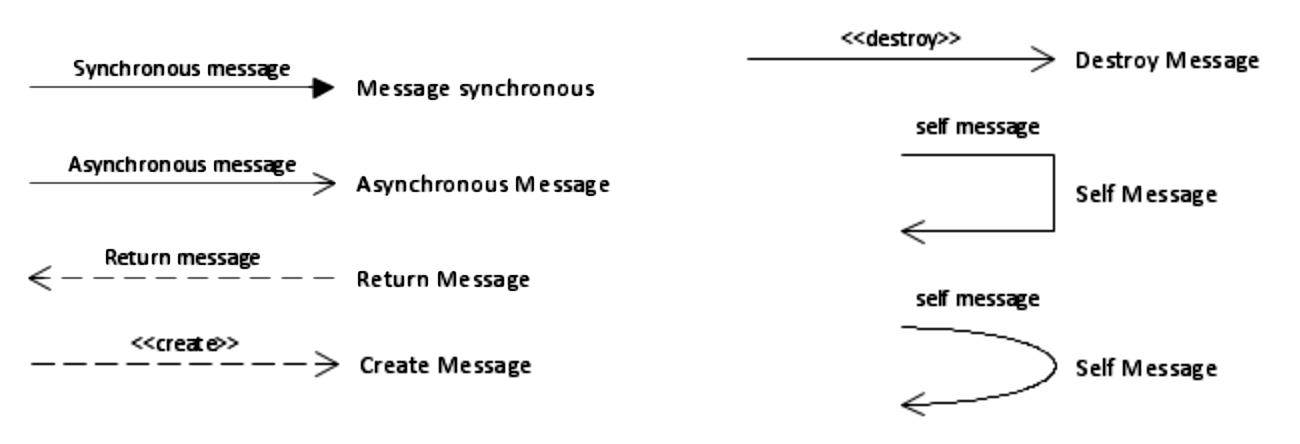
\includegraphics[scale=0.5]{seq-not.png}\\
\end{center}


\subsubsection{Frammenti di interazione}

Oltre al semplice scambio di messaggi \`e possibile rappresentare flussi di esecuzione non lineari come alternative (if-then-else), cicli o parallelismo. Questo avviene attraverso l'uso di \textit{frammenti di interazione} rappresentati da rettangoli con un \textit{operatore di interazione} posto nell'angolo in alto a sinistra. Esempi di operatori di interazione sono:  \textit{alt} (opzioni, come un costrutto if-then-else),  \textit{loop} (cicli),  \textit{opt} (if-then) e  \textit{par} (parallelismo). 

Di seguito un esempio di alt e loop.
\vspace{0.5cm}

\begin{center}
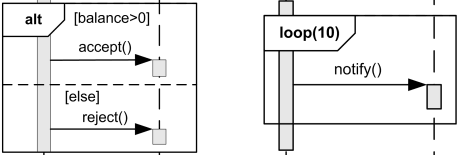
\includegraphics[scale=4.0]{seq-frag.png}\\
\end{center}
\newpage
\section{Example problem}

Si crei un opportuno class diagram per rappresentare una versione semplificate del gioco degli scacchi. Sapendo che:

\begin{enumerate}
\item Si ha una griglia 8x8 denominata Scacchiera 

\item Ogni elemento della griglia si chiama Casella 

\item In ogni casella ci pu\`o essere al pi\`u un Pezzo 

\item I pezzi possono essere: Torre, Cavallo, Alfiere, Regina, Re, ognuno con differenti 
capacit\`a di movimento (si ignori il Pedone per il momento). 

\item La scacchiera viene creata con dei pezzi dentro le caselle posizionati 
opportunamente. 

\item Una casella pu\`o essere vuota o avere un pezzo al suo interno. 

\item Un pezzo pu\`o appartenere al giocatore Bianco o al giocatore Nero e pu\`o spostarsi 
da una casella ad un’altra secondo determinate regole dipendenti dal pezzo. 

\item Un pezzo pu\`o muoversi solo verso una casella vuota od una casella occupata da 
un pezzo avversario. In questo secondo caso il pezzo avversario viene rimosso. I movimenti consentono di spostarsi di al pi\`u una casella in orizzontale, verticale o obliquo.
\end{enumerate}

Si descriva il sequence diagram che consente di effettuare un movimento.
Si implementi un primo prototipo dell'applicazione.

\subsection{UML diagrams}

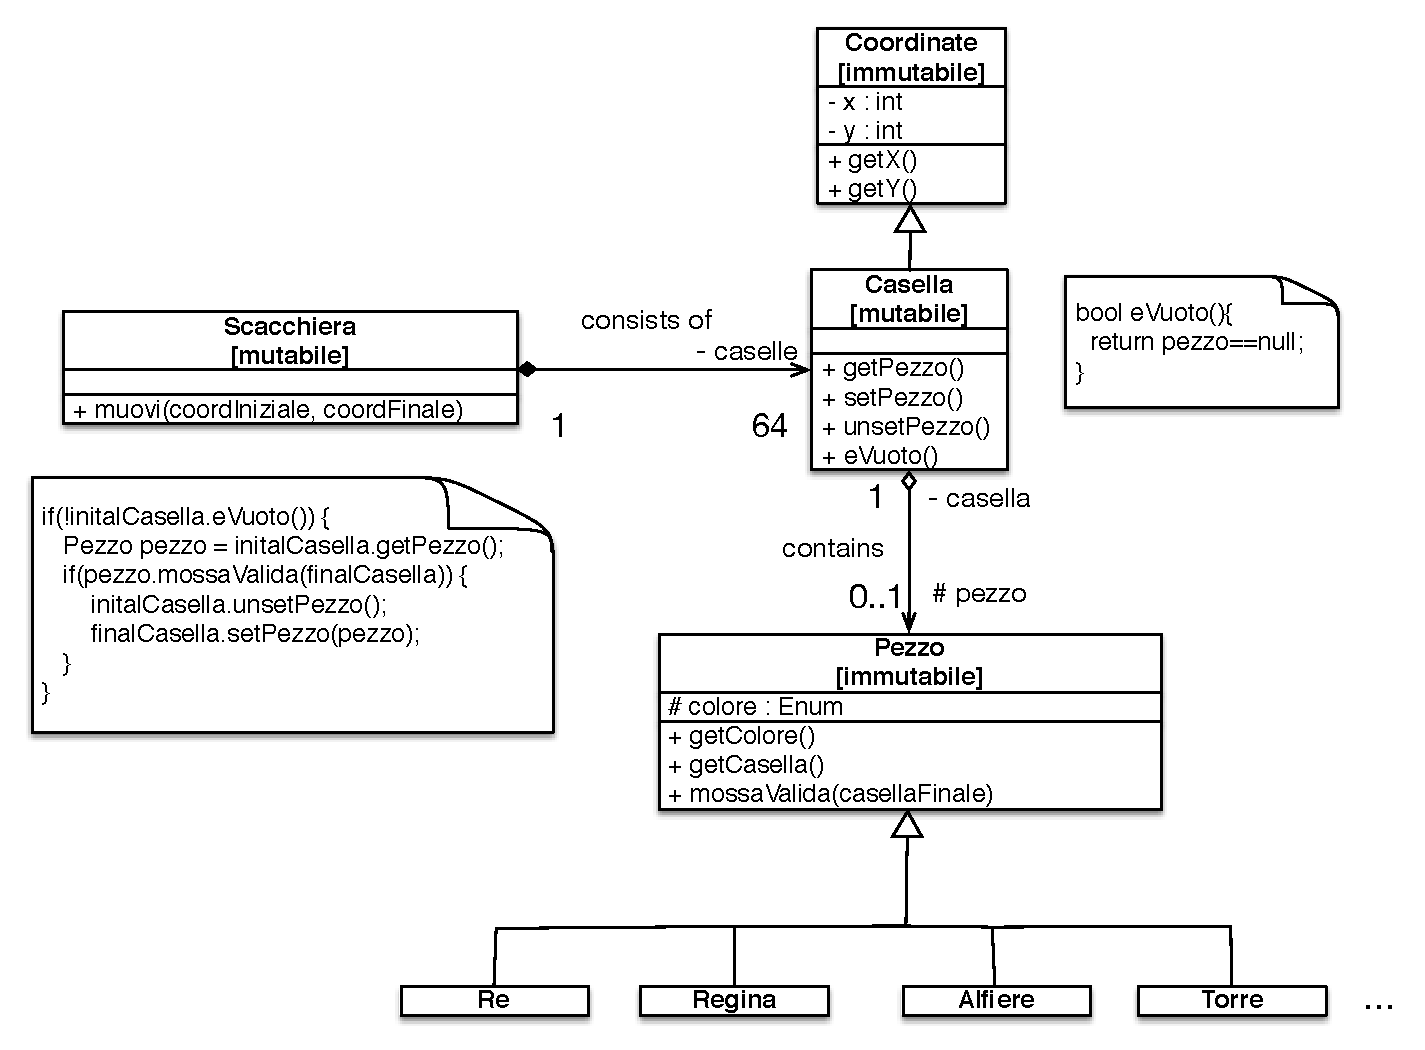
\includegraphics[scale=0.6]{uml-fig.pdf}\\
\vspace{1cm}
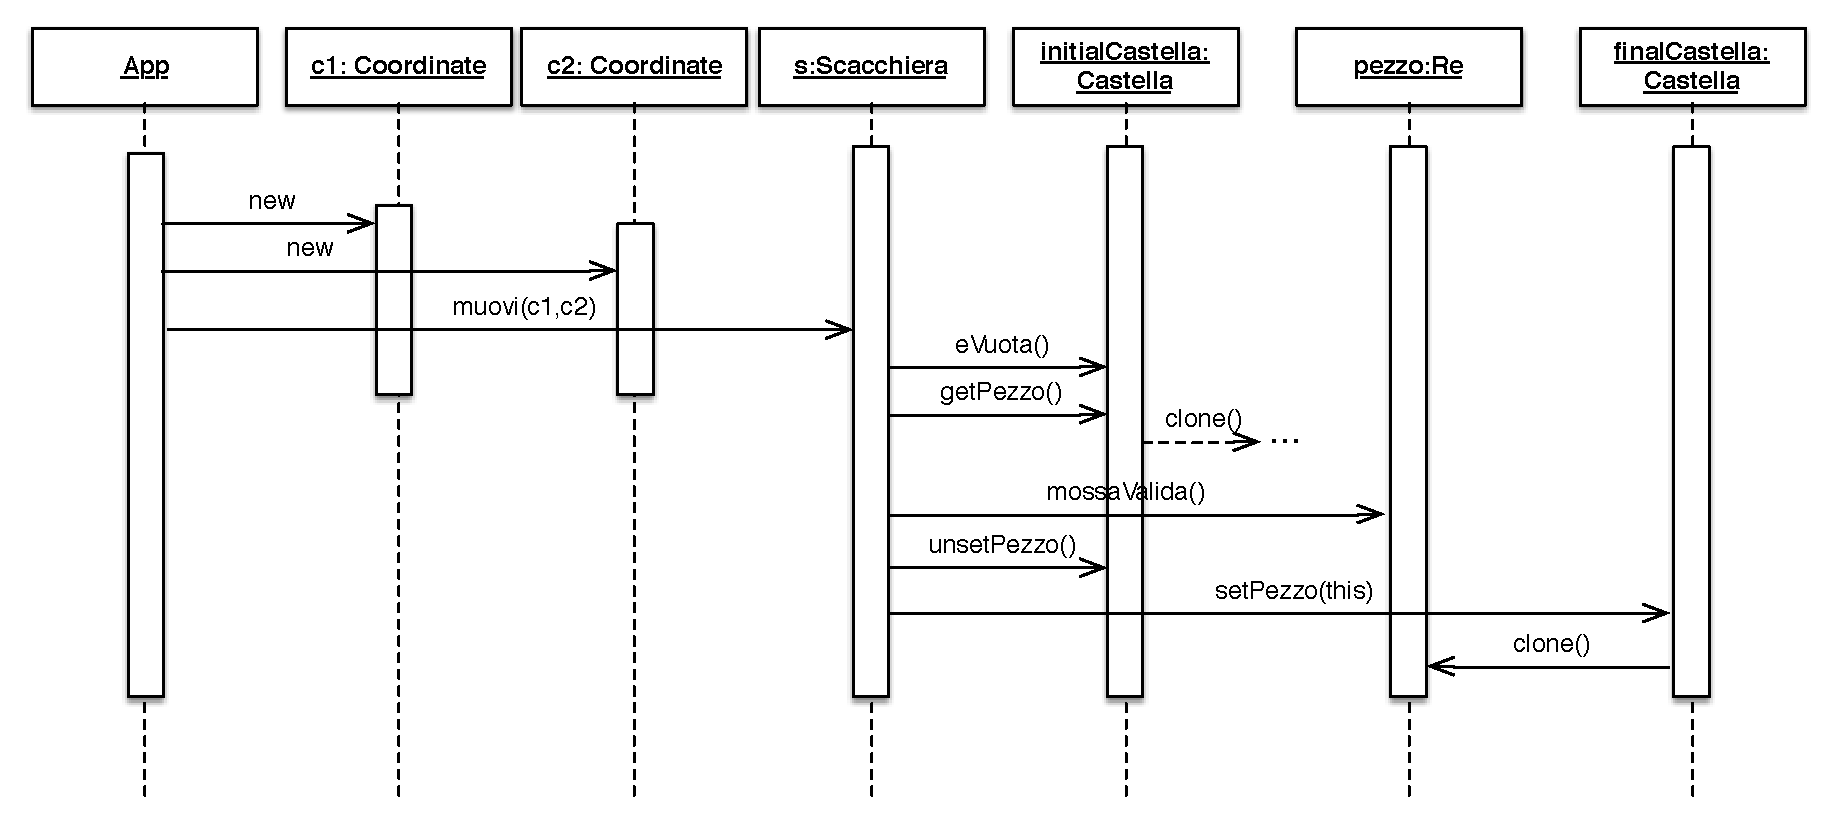
\includegraphics[scale=0.55]{seq-fig.pdf}
\newpage

\subsection{Mapping to Java}

\subsubsection{Coordinate class}
\begin{lstlisting}
 package com.polimi.scacchi;

 public class Coordinate {
 
 	/**
 	 * the x coordiante
 	 */
 	private int x;
 	/**
 	 * the y coordiante
 	 */
 	private int y;
 	 	
 	/**
 	 * Constructor for the Coordinate class
 	 * @param x - x coordinate
 	 * @param y - y coordinate
 	 */
 	public Coordinate(int x, int y){
 		this.x=x;
 		this.y=y;
 	}
 	/**
 	 * @return the x
 	 */
 	public int getX() {
 		return x;
 	}
 	/**
 	 * @param x the x to set
 	 */
 	public void setX(int x) {
 		this.x = x;
 	}
 	/**
 	 * @return the y
 	 */
 	public int getY() {
 		return y;
 	}
 	/**
 	 * @param y the y to set
 	 */
 	public void setY(int y) {
 		this.y = y;
 	}	
 }
 
\end{lstlisting}

\newpage

\subsubsection{Casella class}
\begin{lstlisting}
package com.polimi.scacchi;

public class Casella extends Coordinate {	
	
	/**
	 * Currently placed piece, null if empty
	 */
	private Pezzo pezzo;
	
	/**
	 * Constructor for the Casella class
	 * @param x - x coordinate
	 * @param y - y coordinate
	 */
	public Casella(int x, int y){
		super(x,y);
	}
	
	/**
	 * @return the pezzo
	 */
	public Pezzo getPezzo() {
		if(pezzo!=null)	
			return pezzo.clone();
		return null;
	}

	/**
	 * @param pezzo the pezzo to set and update the pezzo reference to casella
	 */
	public void setPezzo(Pezzo pezzo) {
		if(pezzo==null){
			throw new IllegalArgumentException("The pezzo to be added in the casella cannot be null");
		}
		this.pezzo = pezzo.clone();
	}	
	
	/**
	 * removes the pezzo from the casella (if any)
	 */
	public void unsetPezzo() {
		this.pezzo = null;
	}	
	/**
	 * Checks if the field is empty
	 * @return True if the field is empty, False otherwise
	 */
	public boolean eVuoto(){
		return this.pezzo==null;
	}


	/**
	 * @return the string that describes the Casella object
	 */
	@Override
	public String toString() {
		if(this.eVuoto())
		{
			return " ";
		}
		else
		{
			return this.pezzo.toString();
		}
	}
}
\end{lstlisting}

\subsubsection{Pezzo class}
\begin{lstlisting}
package com.polimi.scacchi;

public abstract class Pezzo {	
	
	/**
	 * the color of the piece
	 */
	protected Colore colore;	
	/**
	 * The current field where the piece is placed, null if nowhere
	 */
	protected Casella casella;
	
	public Pezzo(Colore colore,Casella casella){
		if(colore==null){
			throw new IllegalArgumentException("Il colore del pezzo non deve essere nullo");
		}
		if(casella==null){
			throw new IllegalArgumentException("La casella iniziale del pezzo non deve essere nulla");
		}
		this.colore =colore;
		this.casella=casella;
	}	
	/**
	 * Abstract method  that checks if it is allowed to move a certain piece
	 * @param casellaFinale - the target field where we want to move the piece
	 * @return True if it is allowed to move the piece according to the rules 
	 * of the game, false otherwise
	 */
	public abstract boolean mossaValida(Casella casellaFinale);
	/**
	 * @return the casella
	 */
	public Casella getCasella() {
		return casella;
	}
	/**
	 * @return the colore
	 */
	public Colore getColore() {
		return colore;
	}	
	@Override
	public abstract Pezzo clone();
}
\end{lstlisting}

\subsubsection{Re class}
\begin{lstlisting}
package com.polimi.scacchi;

public class Re extends Pezzo {

	public Re(Colore colore, Casella casella) {
	
		super(colore,casella);
	}

	/* (non-Javadoc)
	 * @see com.polimi.scacchiera.Scacchiera.Pezzo#mossaValida(com.polimi.scacchiera.Scacchiera.Casella)
	 */
	@Override
	public boolean mossaValida(Casella casellaFinale) {
		if(casellaFinale==null){
			throw new IllegalArgumentException("La casella finale della mossa non deve essere nulla");
		}
		
		//cannot go to the field already occupied by a piece with the same color
		if(!casellaFinale.eVuoto()) {
			if(casellaFinale.getPezzo().getColore()==this.getColore()) {
				return false;
			}
		}
		return Math.abs(this.getCasella().getX()-casellaFinale.getX())<=1 &&
				Math.abs(this.getCasella().getY()-casellaFinale.getY())<=1;
	}
	@Override
	public Re clone(){
		return new Re(this.colore, this.casella);
	}

	/**
	 * Prints the piece
	 */
	@Override
	public String toString() {
		return "K";		
	}
}
\end{lstlisting}

\subsubsection{Scacchiera class}
\begin{lstlisting}
package com.polimi.scacchi;

public class Scacchiera {
	/**
	 * 8x8 Matrix of caselle
	 */
	private Casella[][] caselle;

	private static final int SIZE = 8;

	/**
	 * Constructor for Scacchiera, initializes all the fields.
	 */
	public Scacchiera() {
		//initialize fields
		caselle = new Casella[SIZE][SIZE];
		for(int i=0;i<SIZE;i++) {
			for(int j=0;j<SIZE;j++) {
				caselle[i][j]= new Casella(i,j);
			}
		}
				
		//set pieces
		caselle[0][4].setPezzo(new Re(Colore.BLACK,caselle[0][4]));
		//etc...
		
	}
	
	/** 
	 * @see java.lang.Object#toString()
	 */
	@Override
	public String toString(){
		String ret="";
        
    	ret+="---------------------------------\n";

        for(int i=0;i<SIZE;i++)
		{
			ret+="| ";
			for(int j=0;j<SIZE;j++)
			{
				ret+=caselle[i][j].toString();
				ret+=" | ";
				
			}
			ret+="\n";
			ret+="---------------------------------\n";
		}
		
		ret+="\n ";
		return ret;
	}
	
	/**
	 * Moves a piece from one field to another
	 * @param ci - coordinates of the inital field
	 * @param cf - coordinates of the final field
	 */
	public void muovi(Coordinate ci, Coordinate cf){
		if(ci==null){
			throw new IllegalArgumentException("Le coordinate iniziali del pezzo non possono essere nulle");
		}
		if(cf==null){
			throw new IllegalArgumentException("Le coordinate finali del pezzo non possono essere nulle");
		}
		if(ci.getX() >= 0  && cf.getX() >= 0 && 
		   ci.getX() < SIZE && cf.getX() < SIZE &&
		   ci.getY() >= 0  && cf.getY() >= 0 && 
		   ci.getY() < SIZE && cf.getY() < SIZE)
		{
			Casella initalCasella = caselle[ci.getX()][ci.getY()];
			Casella finalCasella = caselle[cf.getX()][cf.getY()];
						
			if(!initalCasella.eVuoto()) {
				Pezzo pezzo = initalCasella.getPezzo();
				if(pezzo.mossaValida(finalCasella)) {
					initalCasella.unsetPezzo();;
					finalCasella.setPezzo(pezzo);
				}
			}
		}
	}	
	
}
\end{lstlisting}

\subsubsection{Main class}
\begin{lstlisting}
package com.polimi.scacchi;

public class App 
{
    public static void main( String[] args )
    {
    	
        Scacchiera s = new Scacchiera();
        System.out.println(s.toString());
        s.muovi(new Coordinate(0, 4), new Coordinate(1, 5));
        System.out.println(s.toString());
        s.muovi(new Coordinate(1, 5), new Coordinate(5, 5));
        System.out.println(s.toString());
    }
\end{lstlisting}

 \subsubsection{Output}
 \begin{lstlisting}
-------------------------
|   |   |   |   | K|    |   |   | 
-------------------------
|   |   |   |   |   |   |   |   | 
-------------------------
|   |   |   |   |   |   |   |   | 
-------------------------
|   |   |   |   |   |   |   |   | 
-------------------------
|   |   |   |   |   |   |   |   | 
-------------------------
|   |   |   |   |   |   |   |   | 
-------------------------
|   |   |   |   |   |   |   |   | 
-------------------------
|   |   |   |   |   |   |   |   | 
-------------------------
 
 
-------------------------
|   |   |   |   |   |   |   |   | 
-------------------------
|   |   |   |   |   | K|    |   | 
-------------------------
|   |   |   |   |   |   |   |   | 
-------------------------
|   |   |   |   |   |   |   |   | 
-------------------------
|   |   |   |   |   |   |   |   | 
-------------------------
|   |   |   |   |   |   |   |   | 
-------------------------
|   |   |   |   |   |   |   |   | 
-------------------------
|   |   |   |   |   |   |   |   | 
-------------------------
 
 
-------------------------
|   |   |   |   |   |   |   |   | 
-------------------------
|   |   |   |   |   | K|    |   | 
-------------------------
|   |   |   |   |   |   |   |   | 
-------------------------
|   |   |   |   |   |   |   |   | 
-------------------------
|   |   |   |   |   |   |   |   | 
-------------------------
|   |   |   |   |   |   |   |   | 
-------------------------
|   |   |   |   |   |   |   |   | 
-------------------------
|   |   |   |   |   |   |   |   | 
-------------------------
\end{lstlisting}



\end{document}

